\documentclass{standalone}
\usepackage{tikz}
\usepackage{ctex,siunitx}
\setCJKmainfont{Noto Serif CJK SC}
\usepackage{tkz-euclide}
\usepackage{amsmath}
\usetikzlibrary{patterns, calc,3d}
\usetikzlibrary {decorations.pathmorphing,decorations.pathreplacing,decorations.shapes}
\tikzset{label style/.append style={font=\small}}
\begin{document}
\small
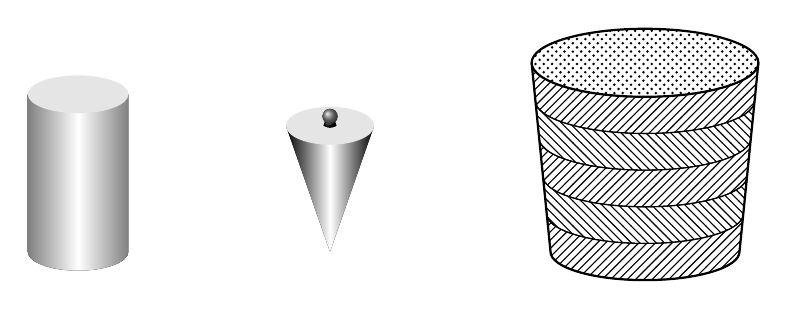
\begin{tikzpicture}[>=latex,scale=0.8]
  \begin{scope}
    \fill[left color=gray,right color=gray,middle color=white](0.8,0)arc(0:-180:0.8 and 0.3)--(-0.8,2.5)--(0.8,2.5)--cycle;
    \fill[lightgray!40](0,2.5)ellipse(0.8 and 0.3);
  \end{scope}
  \begin{scope}[xshift=4cm]
    \fill[left color=black,right color=black,middle color=white](0.7,2)--(-0.7,2)--(0,0)--cycle;
    \fill[lightgray!40](0,2)ellipse(0.7 and 0.3);
    \fill[ball color=black](0.1,2)arc(0:180:0.1)to[bend right](0.1,2)--cycle;
    \fill[ball color=gray](0,2.15) circle(0.12);
  \end{scope}
  \begin{scope}[xshift=9cm]
    \foreach \x in {0,1.2,2.4}
    {
      \draw[pattern=north east lines](1.5+\x*0.1,\x)arc(0:-180:{1.5+\x*0.1} and {0.45+\x*0.03})--(-1.56-\x*0.1,\x+0.6)arc(-180:0:{1.56+\x*0.1} and {0.468+\x*0.03})--cycle;
    }
    \foreach \x in {0.6,1.8}
    {
      \draw[pattern=north west lines](1.5+\x*0.1,\x)arc(0:-180:{1.5+\x*0.1} and {0.45+\x*0.03})--(-1.56-\x*0.1,\x+0.6)arc(-180:0:{1.56+\x*0.1} and {0.468+\x*0.03})--cycle;
    }
    \draw[thick,pattern=crosshatch dots](0,3)ellipse(1.8 and 0.54);
    \draw[thick](-1.8,3)--(-1.5,0)arc(180:360:1.5 and 0.45)--(1.8,3);
  \end{scope}
\end{tikzpicture}
\end{document}